\documentclass{report}

% \usepackage[tmargin=2.5cm,rmargin=3cm,lmargin=3cm,bmargin=3cm]{geometry} 
% Top margin, right margin, left margin, bottom margin, footnote skip
\usepackage[utf8]{inputenc}
\usepackage{biblatex}
\addbibresource{./reference.bib}
% linktocpage shall be added to snippets.
\usepackage{hyperref,theoremref}
\hypersetup{
	colorlinks, 
	linkcolor={red!40!black}, 
	citecolor={blue!50!black},
	urlcolor={blue!80!black},
	linktocpage % Link table of content to the page instead of the title
}

\usepackage{blindtext}
\usepackage{tikz}
\usetikzlibrary{cd}
\usetikzlibrary{positioning}

\usepackage{amssymb}
\usepackage{mathtools}
\usepackage{titlesec}
\usepackage{amsthm}
\usepackage{thmtools}
\usepackage{amsmath}
\usepackage{amssymb}
\usepackage{graphicx}
\usepackage{titlesec}
\usepackage{xcolor}
\usepackage{multicol}
\usepackage{hyperref}
\usepackage{import}


\newtheorem{thm}{Theorema}[chapter]
\newtheorem{lemma}[thm]{Lemma}
\newtheorem{coro}[thm]{Corollarium}
\newtheorem{prop}[thm]{Propositio}
\theoremstyle{definition}
\newtheorem{defn}[thm]{Definitio}

\theoremstyle{definition}
\newtheorem{axiom}[thm]{Axioma}
\newtheorem{observation}[thm]{Observation}

\theoremstyle{remark}
\newtheorem{remark}[thm]{Observatio}
\newtheorem{hypothesis}[thm]{Coniectura}
\newtheorem{example}[thm]{Exampli Gratia}

\renewcommand\emptyset{\varnothing}
\renewcommand\mod{\text{ mod }}
%TODO mayby proof environment shall have more margin
% \renewenvironment{proof}{\vspace{0.4cm}\noindent\small{\emph{Demonstratio.}}}{\qed\vspace{0.4cm}}
% \renewenvironment{proof}{{\bfseries\emph{Demonstratio.}}}{\qed}
\renewcommand\qedsymbol{Q.E.D.}
% \renewcommand{\chaptername}{Caput}
% \renewcommand{\contentsname}{Index Capitum} % Index Capitum 
\renewcommand{\emph}[1]{\textbf{\textit{#1}}}
\renewcommand{\ker}[1]{\operatorname{Ker}{#1}}

%\DeclareMathOperator{\ker}{Ker}

% New Commands
\newcommand{\bb}[1]{\mathbb{#1}} %TODO add this line to nvim snippets
\newcommand{\orb}[2]{\text{Orb}_{#1}({#2})}
\newcommand{\stab}[2]{\text{Stab}_{#1}({#2})}
\newcommand{\im}[1]{\text{im}{\ #1}}
\newcommand{\se}[2]{\text{send}_{#1}({#2})}
\newcommand{\be}{b_\text{eff}}
\renewcommand{\L}{L_{\lambda}(x)}

% project specific macros
% m stands for maximum
\newcommand{\mx}{\overline{x}}


\title{Quantifying Chaos}
\author{Harry Han} 
\date{\today}

\begin{document}
\maketitle
\tableofcontents
\chapter{What is Chaos}
% Listing the definition of chaos

\section{Example of Chaos}

\begin{defn}[Logistic Map]
	The logistic map $L(x; \lambda): [0,1] \rightarrow [0,1]$ is a quadratic map depending on the parameter $\lambda$ defined as 
	\begin{equation} \label{logistic_map}
		L(x; \lambda) = 4\lambda x(1 -x ),
	\end{equation}
	where $0\leq \lambda \leq 1$.
\end{defn}

\section{Devaney's Definition}

\begin{defn}[Topologically Transitive]
	Let $J$ be a set with a topology.
	The function $f: J \rightarrow J$ is topologically transitive, if for all non-empty open sets $U_1, U_2 \in J$, there exist $k \in \bb{N}$ such that $f^k(U_1) \cap U_2 \neq \varnothing$. 
	Here $f^k$ denotes the composition $\underbrace{f \circ f \cdots \circ f}_{k \text{ times}}$
\end{defn}

\begin{defn}[Dense]
	Let $X$ be subset of the topological space $J$. 
	$X$ is dense if $\overline{X} = J$, where $\overline{X}$ denote the closure of $X$.
\end{defn}

\begin{defn}[Periodic Point]
	A point $x$ is a period of period $k$ if $f^k(x)=x$.
\end{defn}

\begin{defn}[Sensitive Dependence on Initial Condition]
	Let $J$ be a metric space with the metric $d: J \times J \rightarrow \bb{R}$.

	$f: J \rightarrow J$ has sensitive dependence on initial condition if there exists some $\delta > 0$ such that for all $x \in J$ and any neighbourhood $X$ containing $x$, there exists $y \in X$ and $n \in \bb{N}$ such that $d(f^n(x), f^n(y)) > \delta$.
\end{defn}

\begin{defn}[Chaos, Devaney's Definition]\label{def:Devaney_definition_for_chaos}
	Let $V$ be a metric space.
	A function $f: V \rightarrow V$ is chaotic if 
	\begin{enumerate}
		\item the set of periodic points are dense in $V$,
		\item $f$ is topologically transitive,
		\item $f$ has sensitive dependence on initial condition. 
	\end{enumerate}
	
\end{defn}


The definition here is attributed to Devaney \cite{Devaney_green_book_chaos_definition}. 
The first two requirements are purely topological, while the last one requires a metric. 
While in most circumstances topological properties are more generalised than the metric properties, here, surprisingly, as long as $V$ is a metric space (which is part of the assumption), the first two implies the third\cite{Banks}. 
As a result, we only need to check the first two conditions to determine if a function is chaotic.

\begin{thm}[Criterion For Chaotic Function]
	Let $V$ be a metric space. 
	Function $f: V \rightarrow V$ is chaotic as defined in \ref{def:Devaney_definition_for_chaos}
	if and only if its the periodic points are dense $V$ and it is topologically transitive,
\end{thm}

% TODO: Say more about doubling map. 
% TODO: graph, say more in introduction, etc?
% The doubling map is topologically transitive to the map in $S^1$

\begin{example}\label{ex_doubling_map}
	Recall the doubling map $f: [0,1) \rightarrow [0,1)$
	$$
	f(x) = 
		\begin{cases}
			2x &\text{ if } 2x < 1 \\
			2x -1 &\text{ if } 2x > 1
		\end{cases}
	$$
	% TODO: more explanation
	This map can also be regarded as doubling the angles on the unit cycle: $g: S^1 \rightarrow S^1$ given by $ g(\theta) = 2 \theta$.
	
	The doubling map is \textit{chaotic}.

	All non-zero rational points $\frac{p}{q} \in [0,1)$ with odd denominater are periodic points for $f$. 
	The set of these points are dense.
	To show the periodicity, note the images of $\frac{p}{q}$ under repetitive applications of $f$ are $\frac{p}{q}, \frac{2p}{q}, \cdots, \frac{2^k p}{q}, \cdots$.
	We can regard all the numerators as the equivalence classes module $q$.
	Since this sequence is infinite and there are only finitely many possibilities for the numerators, some of the numerators must coincide. Let them be $2^k p$ and $2^{k'} p$. 
	Without loss of generacity let $k > k'$, and
	$$
	2^k p \equiv 2^{k'} p \mod q \implies 
	2^{k-k'} p \equiv p \mod q \text{ (as $q$ is odd)},
	$$
	which measn $f^{k-k'}(\frac{p}{q}) = \frac{p}{q}$, i.e., $\frac{p}{q}$ is a point of period $k - k'$.

	To show $f$ is topologically transitive is even easier. 
	For any non-empty open set $U \in [0,1)$, by definition there exists an open interval $J = (x, x+ \delta) \subseteq U$. 
	$J$ has diameter $\delta$, $f(J)$ has diameter $2 \delta$, and $f^k(J)$, $2^k \delta$. 
	Since the length of $[0,1)$ is $1$, after some finite iteration $f^k(J)$ would covers all of $[0,1)$ and intersect any other open sets.

	By generalising this proof it is clear any maps in the form 
	$$
	g: S^1 \rightarrow S^1; g(\theta) = r \theta, r \in R
	$$
	are chaotic.
\end{example}

To prove the doubling map is chaotic is a gentle exercise. 
To directly find the points of periodicity and prove that a general function is topologically transitive is difficult.
Instead, we can circumvent these challenges by exploiting certain topological properties introduced in the next section.

\section{Topological Conjugacy}

\begin{defn}[Topological Conjugacy]
Funcitons $f: X \rightarrow X$, $g:  Y \rightarrow Y$ are topologically conjugate if there exist a homeomorphism $\phi: X \rightarrow Y$ such that 
$\phi \circ f = g \circ \phi$,
i.e, the following diagram commutes.
\begin{center}
    \begin{tikzcd}
        X \arrow[r, "f"] \arrow[d, "\phi" swap] & X \arrow[d, "\phi"] \\
        Y \arrow[r, "g"] & Y
    \end{tikzcd}
\end{center}

The maps $f,g$ are semiconjugate if there exists a continuous surjection, $\psi$ such that $\psi \circ f = g \circ \psi$.
\end{defn}

% TODO: Shall we introduce a notation for topological conjugacy? 
% no notation is provided by Devaney or Wikipedia

To rephrase a definition, $f,g$ are conjugate if there exists and homeomorphism $\phi$ such that $f = \phi^{-1} \circ g \circ \phi$.
So $f^{n} = \phi^{-1} \circ g^{n} \circ \phi$; that is $f^n$ is conjugate to $g^n$.

Topological conjugacy is an equivalence condition. 
$f$ is conjugate to itself by identity map. 
$\phi \circ f = g \circ \phi$ implies $f \circ \phi^{-1} = \phi^{-1} \circ g$, so $g$ is also conjugate to $f$.
Lastly, if $f$  is conjugate to $g$ via $\phi$, and $g$ is conjugate to $h$ via $\phi'$, $\phi' \circ \phi \circ f = \phi' g \circ \phi = h \circ \phi'' $, which means $f$ is conjugate to $h$ via $h' \circ h$.

Topological semiconjugacy only requires a continuous surjection, $\psi$, such that $\psi \circ f = g \circ \psi$. 
As $\psi$ may not have inverset semiconjugacy can not be an equivalence condition.
Nevertheless, if $f$ is semiconjugate to $g$, so is $f^{k}$ to $g^{k}$ for any $k \in \bb{N}$. 
This is because 
$$
	\psi \circ f\circ \cdots \circ f = g \circ \psi \circ f \cdots \circ f = \cdots = g^k \circ \psi
$$

 % TODO: verify this is true
If $f$ is conjugate to $g$, necessarily $f$ and semi-conjugate to $g$ and $g$ is semiconjugate to $f$. 
However, if $f$ is semiconjugate to $g$ and $g$ is semiconjugate to $f$, $f$ is not necessarily conjugate to $g$. 

Chaotic behaviors are \emph{preserved} by conjugacy.

\begin{thm}[Semiconjugacy preserves Chaos]\label{th_semicong_chaos}
	If $f$ is semiconjugate to $g$ and $f$ is chaotic, $g$ also is.
\end{thm}
% TODO: can g chaotic implies f also is if f is semiconjugate to g?
% FIND counter example

\begin{proof}
	Let $f: X \rightarrow X$, $g:  Y \rightarrow Y$, and let $\psi$ be the promised continuous surjection such that
	$\psi \circ f = g \circ \psi$. 
	Since $\psi$ is conituously surjective, for any non-empty open set $M \in Y$, $\psi^{-1}(M)$ is an non-empty open set in $X$.

	Let us first prove that the set of periodic points of $g$ is ddense.
	For any $x$ such that $f^k(x) = x$, notice that $g^k \circ \psi (x) = \psi \circ f^k (x) = \psi(x)$. 
	This means, if the set of periodic points of $f$ is $X$, $\psi(X)$ is a sub set of the set of periodic point of $g$.

	For the sake of contradiction assuming $\psi(X)$ is not dense in $Y$. 
	This means there is a open set $M \subset Y$ such that $M \cup \psi(X) = \emptyset$.
	The preimage $\psi^{-1}(M)$ is an non-empty open set of $X$, and by assumption, it does not contains any periodic points of $f$, which is a contradiction.

	To prove that $g$ is topologically transitive, consider any non-empty open set $M, N \in Y$, and $\psi^{-1}(M), \psi^{-1}(N)$ are non-empty open set in $X$. 
	By assumption there exists some $k$ such that $f^k(\psi^{-1}(M)) \cap f^k(\psi^{-1}(N)) \neq \emptyset$, this means 
	\begin{align*}
		g^k(M) \cap g^k(N) = \psi \circ f^k(\psi^{-1}(M)) \cap \psi \circ f^k(\psi^{-1}(N)) \\
		\subset \psi( f^k(\psi^{-1}(M)) \cap  f^k(\psi^{-1}(N))) \neq \emptyset
	\end{align*}
\end{proof}

Since conjugacy impies semi-conjugacy on both directions, we have the following important proposition.

\begin{prop}[Conjugacy Class share chaotic behavior]\label{prop_conj_chaos}
	If $f$ is conjugate to $g$, $f$ is chaotic if and only if $g$ is chaotic.
\end{prop}

There are abundant examples of topological conjugacy.

\begin{example}
	If $f$ is conjugate to $g$ via $\phi$, and $g$ is conjugate to $h$ via $\psi$, $f$ is conjugate to $h$ via $\psi \circ \phi$.
	\begin{center}
	    \begin{tikzcd}
	        X \arrow[r, "f"] \arrow[d, "\phi" swap] & X \arrow[d, "\phi"] \\
	        Y \arrow[r, "g"] \arrow[d, "\psi" swap] & Y \arrow[d, "\psi"] \\
	        Z \arrow[r, "h"] & Z \\
	    \end{tikzcd}
	\end{center}
\end{example}

\begin{example}
	For open interval $[-\epsilon_1, \epsilon_2] \in \bb{R}$. 
	$f: [-\epsilon_1, \epsilon_2] \rightarrow [-\epsilon_1, \epsilon_2]$
	is conjugate to 
	$g: [-\epsilon_1 + a, \epsilon_2 + a] \rightarrow  [-\epsilon_1 + a, \epsilon_2 + a]$
	where $g(x)= f(x -a) + a$ via $\phi(x) = x + a$.

	For a concrete example, consider the map 
	$f: [0,1] \rightarrow [0,1]$
	defined as $f(x) = 4x(1-x)$,
	which is conjugate to 
	$g(x): [-\frac{1}{2}, \frac{1}{2}] \rightarrow [-\frac{1}{2}, \frac{1}{2}]$
	defined as $g(x) = -4x^2 + \frac{1}{2}$ 
	through $\phi(x) = x -\frac{1}{2}$, i.e., $ \phi \circ f=  g \circ \phi$.
\end{example}

\begin{example}
	For closed interval $[-\epsilon_1, \epsilon_2] \in \bb{R}$. 
	$f: [-\epsilon_1, \epsilon_2] \rightarrow [-\epsilon_1, \epsilon_2]$
	is conjugate to 
	$g: [-\frac{\epsilon_1}{a}, \frac{\epsilon_2}{a}] \rightarrow [-\frac{\epsilon_1}{a}, \frac{\epsilon_2}{a}]$
	where $g(x)= \frac{1}{a}(ax)$ via $\phi(x) = ax$.


	As another concrete example, the map $f: [0,1] \rightarrow [0,1]$
	defined as $f(x) = -4x^2 + \frac{1}{2})$,
	is conjugate to 
	$g(x): [-1, 1] \rightarrow [-1, 1]$
	defined as $g(x) = 2x^2 - 1$
	through $\phi(x) = -2x$.
\end{example}

\begin{example}
	Consider the doubling map $f: [0,\pi) \rightarrow [0, \pi)$ defined thus: 
	$$
	f(\theta) = 
		\begin{cases}
			2 \theta &\text{ if } 2x <  \pi \\
			2 \theta - \pi &\text{ if } 2x > \pi
		\end{cases}
	$$
	
	This map is doubling the angle of the unit circle.

	$f$ is semi-conjugate to $g: [-1, 1] \rightarrow [-1, 1]$ defined as $g(x) = 2x^2 - 1$ through $\cos(x)$.

	Example \ref{ex_doubling_map} shows that the doubling map is chaotic, so is $g$.
\end{example}

\begin{example}\label{ex_logistic_at_4}\label{ex_logistic_and_doubling}
	The above 3 examples shows that the doubling map is semi-conjugate to the logistic map $L_1(x) = 4x(1-x)$.
\end{example}

\begin{example}
	The logistic map $L_1(x) = 4x(1-x)$ in the interval $[0,1]$ is topologically conjugate to the tent map defined as 
	\begin{equation}
		f(x) = 
		\begin{cases}
			2x   &\text{ if } 0<x \leq \frac{1}{2} \\ 
			2-2x &\text{ if } \frac{1}{2} < x \leq 1
		\end{cases}
	\end{equation}
	via the map $h: [0,1] \rightarrow [0,1]$ defined as $h(x) = \sin^2(\frac{\pi x}{2})$.
	This can be verified by the simple computation $L_1 \circ h = h \circ f$.
\end{example}

\chapter{Bifurcations in Discrete Dynamical Systems}

\section{The Logistic Map as Model for Population Growth}

One dimensional recursive equations $x_{n+1} = f(x_n)$ are used for modeling various dynamical systems. 
Its simplicity makes it easy to study, and many of its properties are also inherited by their more complicated counterparts.

Consider, for example, bacteria population in discrete time intervals. 
If the population is low and resource abundant, the rate of growth is in porportion to the population, which give rise to the following equation

$$
p_{t+1} = p_{t} b,
$$
where $p_{t}$ is the population of the bacteria at the dicrete time $t$ and $b$ as a constant is the static birth rate for bacteria whose value will depend on the model.

The limited resource will slow down the rate of growth as the population increases, and the the relation will become 

$$
	p_{t+1} =  p_{t} \be
$$

The usual assumption is that $\be$ is close to $b$ when the population is closed to zero, and there is a threshold which the population will never surpass. At the threshold $\be$ will be zero.

The simplest equation for modelling $\be$ is the linear equation

$$
\be = b - ap,
$$

where $a$ is another constant.
Combining the two, the recursive formula becomes 

$$
p_{t+1}  = b p_t - ap_t^2
$$

Substituting $p_{t} := \frac{b}{a} x_{t}, \lambda := \frac{b}{4}$, we obtain

$$
x_{t+1} = 4 \lambda x_t(1-x_t) 
$$

Indeed, thence come the standard forms of the logistic map

\begin{equation}\label{eq_logistic}
	L_{\lambda}(x) = 4 \lambda x(1-x)
\end{equation}

% graph produced by `logistic_map_diff_lambda`
\begin{figure}[t]
	\centering
	\label{fig:logistic_map_diff_lambda}
	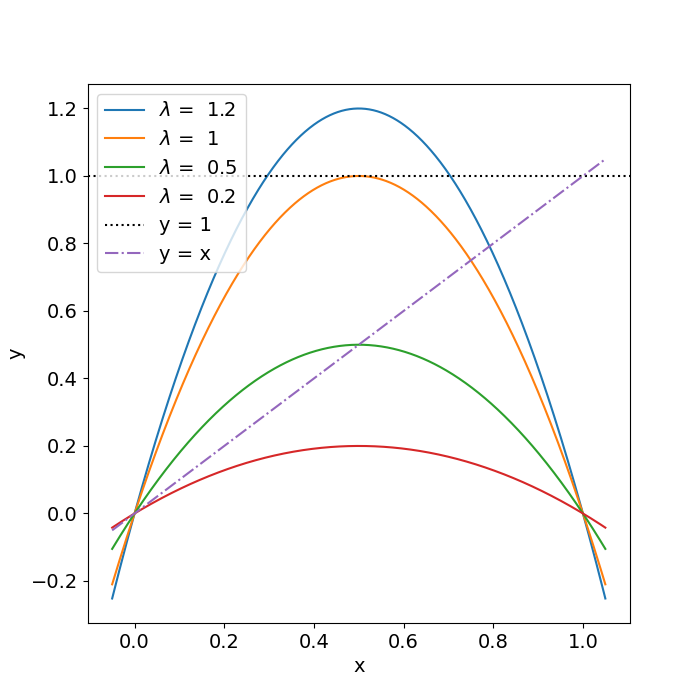
\includegraphics[width=0.7\textwidth]{./figures/logistic_map_diff_lambda.png}
	\caption{Graphs of logistic map $L_{\lambda}(x) = 4 \lambda x(1-x)$ for different $\lambda$ compared with the line $y=x$ and $y = 1$.} 
\end{figure}


For our purpose the restriction $\lambda >0$ is applied.
Scrutinising the class of discrete logistic functions plotted in figure \ref{fig:logistic_map_diff_lambda}, some of their properties are obvious

\begin{enumerate}
	\item $\L$ is a smooth function.
	\item $\L$ concaves downwards, that is, $\L'' < 0$.
	\item $\L$ attains a unique maximum at $x = \frac{1}{2}$, and $L_{\lambda}(\frac{1}{2}) = \lambda$.
	\item When $0 \leq \lambda$ and $x$ is restricted to the domain $[0, 1]$, $\L$ is a two-to-one non-surjective (except for $\lambda = 1$) function $\L: [0,1] \rightarrow [0,\lambda]$. 
\end{enumerate}

Some sources defined the logistic map as $L'_{\lambda'}(x) = \lambda' x(1-x)$ without the constant 4. 
In this report, however, we will use equation \ref{eq_logistic}, which has the advantage that the maximum value attained by $\L$ is $\lambda$. This notation will also be consistent to the definitions of other class of functions discussed later in the report.

We can check if this model would work as expected by comparing it to its continuous counterpart 

\begin{equation}\label{eq_logistic_continuous}
	\frac{dp}{dt} = c p(x) (1-p(x)),
\end{equation}

whose unique solution with the initial condition $p(0) = \frac{1}{2}$ is 

$$
p(t) = \frac{e^{cx}}{1+e^{cx}}
$$

\begin{figure}[b!]
	\centering
	\label{fig:con_vs_discrete}
	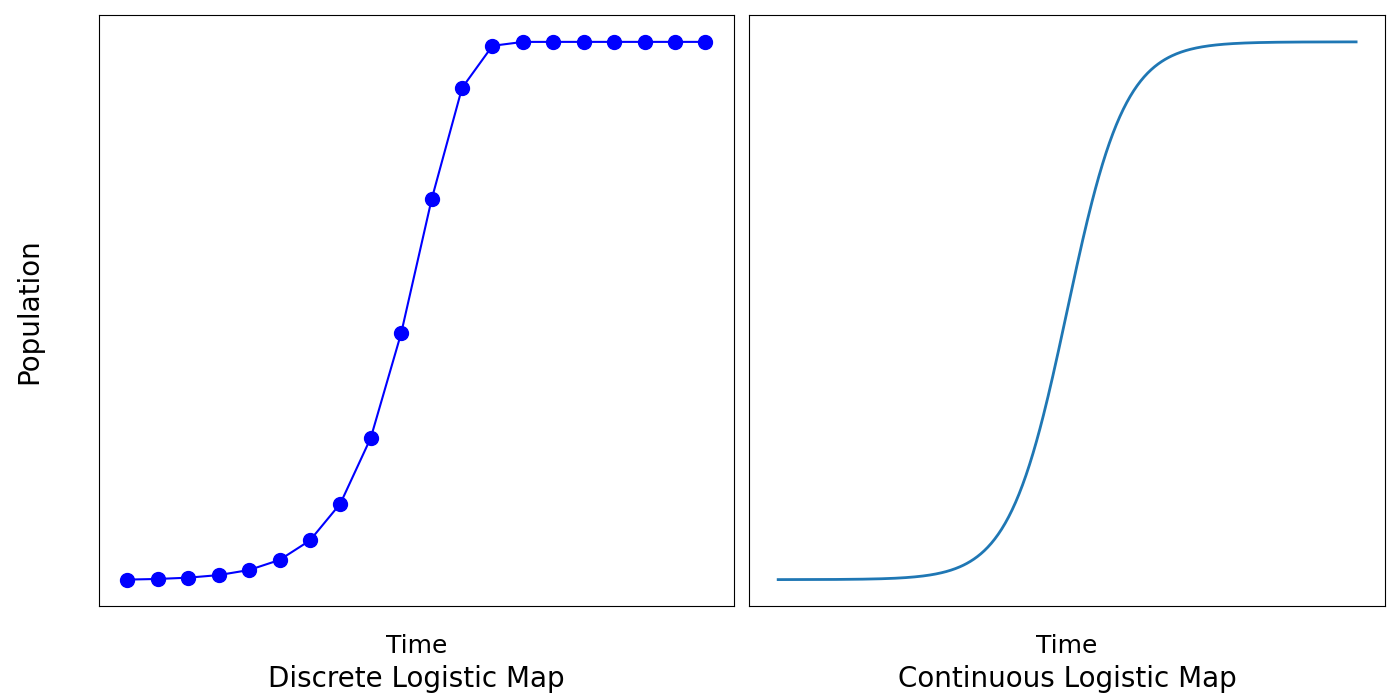
\includegraphics[width=0.8\textwidth]{./figures/con_vs_discrete_logistic_map.png}
	\caption{Discrete (left) v.s. continuous (right) logisitc map. Discrete case is modeld by $\lambda = 0.5$ and $x_0 = 0.0003$. The continuous case has $c=1$.}
\end{figure}

The graph of these two maps are shown in figure \ref{fig:con_vs_discrete}.
The population of the discrete case was obtained by setting an arbitrary initial value, here $x_0 = 0.0003$, and the population of the next time interval was obtained by simple iteration of the logistic map, that is $x_{i+1} = L_{\lambda}(x_i)$.
For the continuous case the population at each time was obtained by solving the differential equation with initial condition.
Indeed, at least for the selected value of $\lambda$ and $c$, the population modeld by the two maps are similar.

Having settled that the discrete logistic map is indeed, at least for some values of $\lambda$, a good simplification for the already-simplified equation \ref{eq_logistic_continuous} as a model for population growth, you may wondered why bother studying such a simple equation. 
The reason is, as simple as it seems, the iteration of equation \ref{eq_logistic} gives rise to some extremely complicated dynamical systems with many surprising properities. 
These interesting dynamics are also observed in the continuous case and is the study of the next session.

% graph produced by logistic_vs_continuous_modelling_population


\section{Logistic Bifurcations}

The first step of studying logistic bifurcations is to plot it with different initial values and $\lambda$. 
For now only $0 \leq \lambda \leq 1$ and $0 \leq x_0 \leq 1$ are considered, so that $\L$ is a map from $[0,1]$ to $[0,1]$. 

% graph produced by `modelling_pop_with_diff_logistic_maps` in `graph_qc` repo
\begin{figure}[htbp]
	\centering
	\label{fig:various_iter_logistic}
	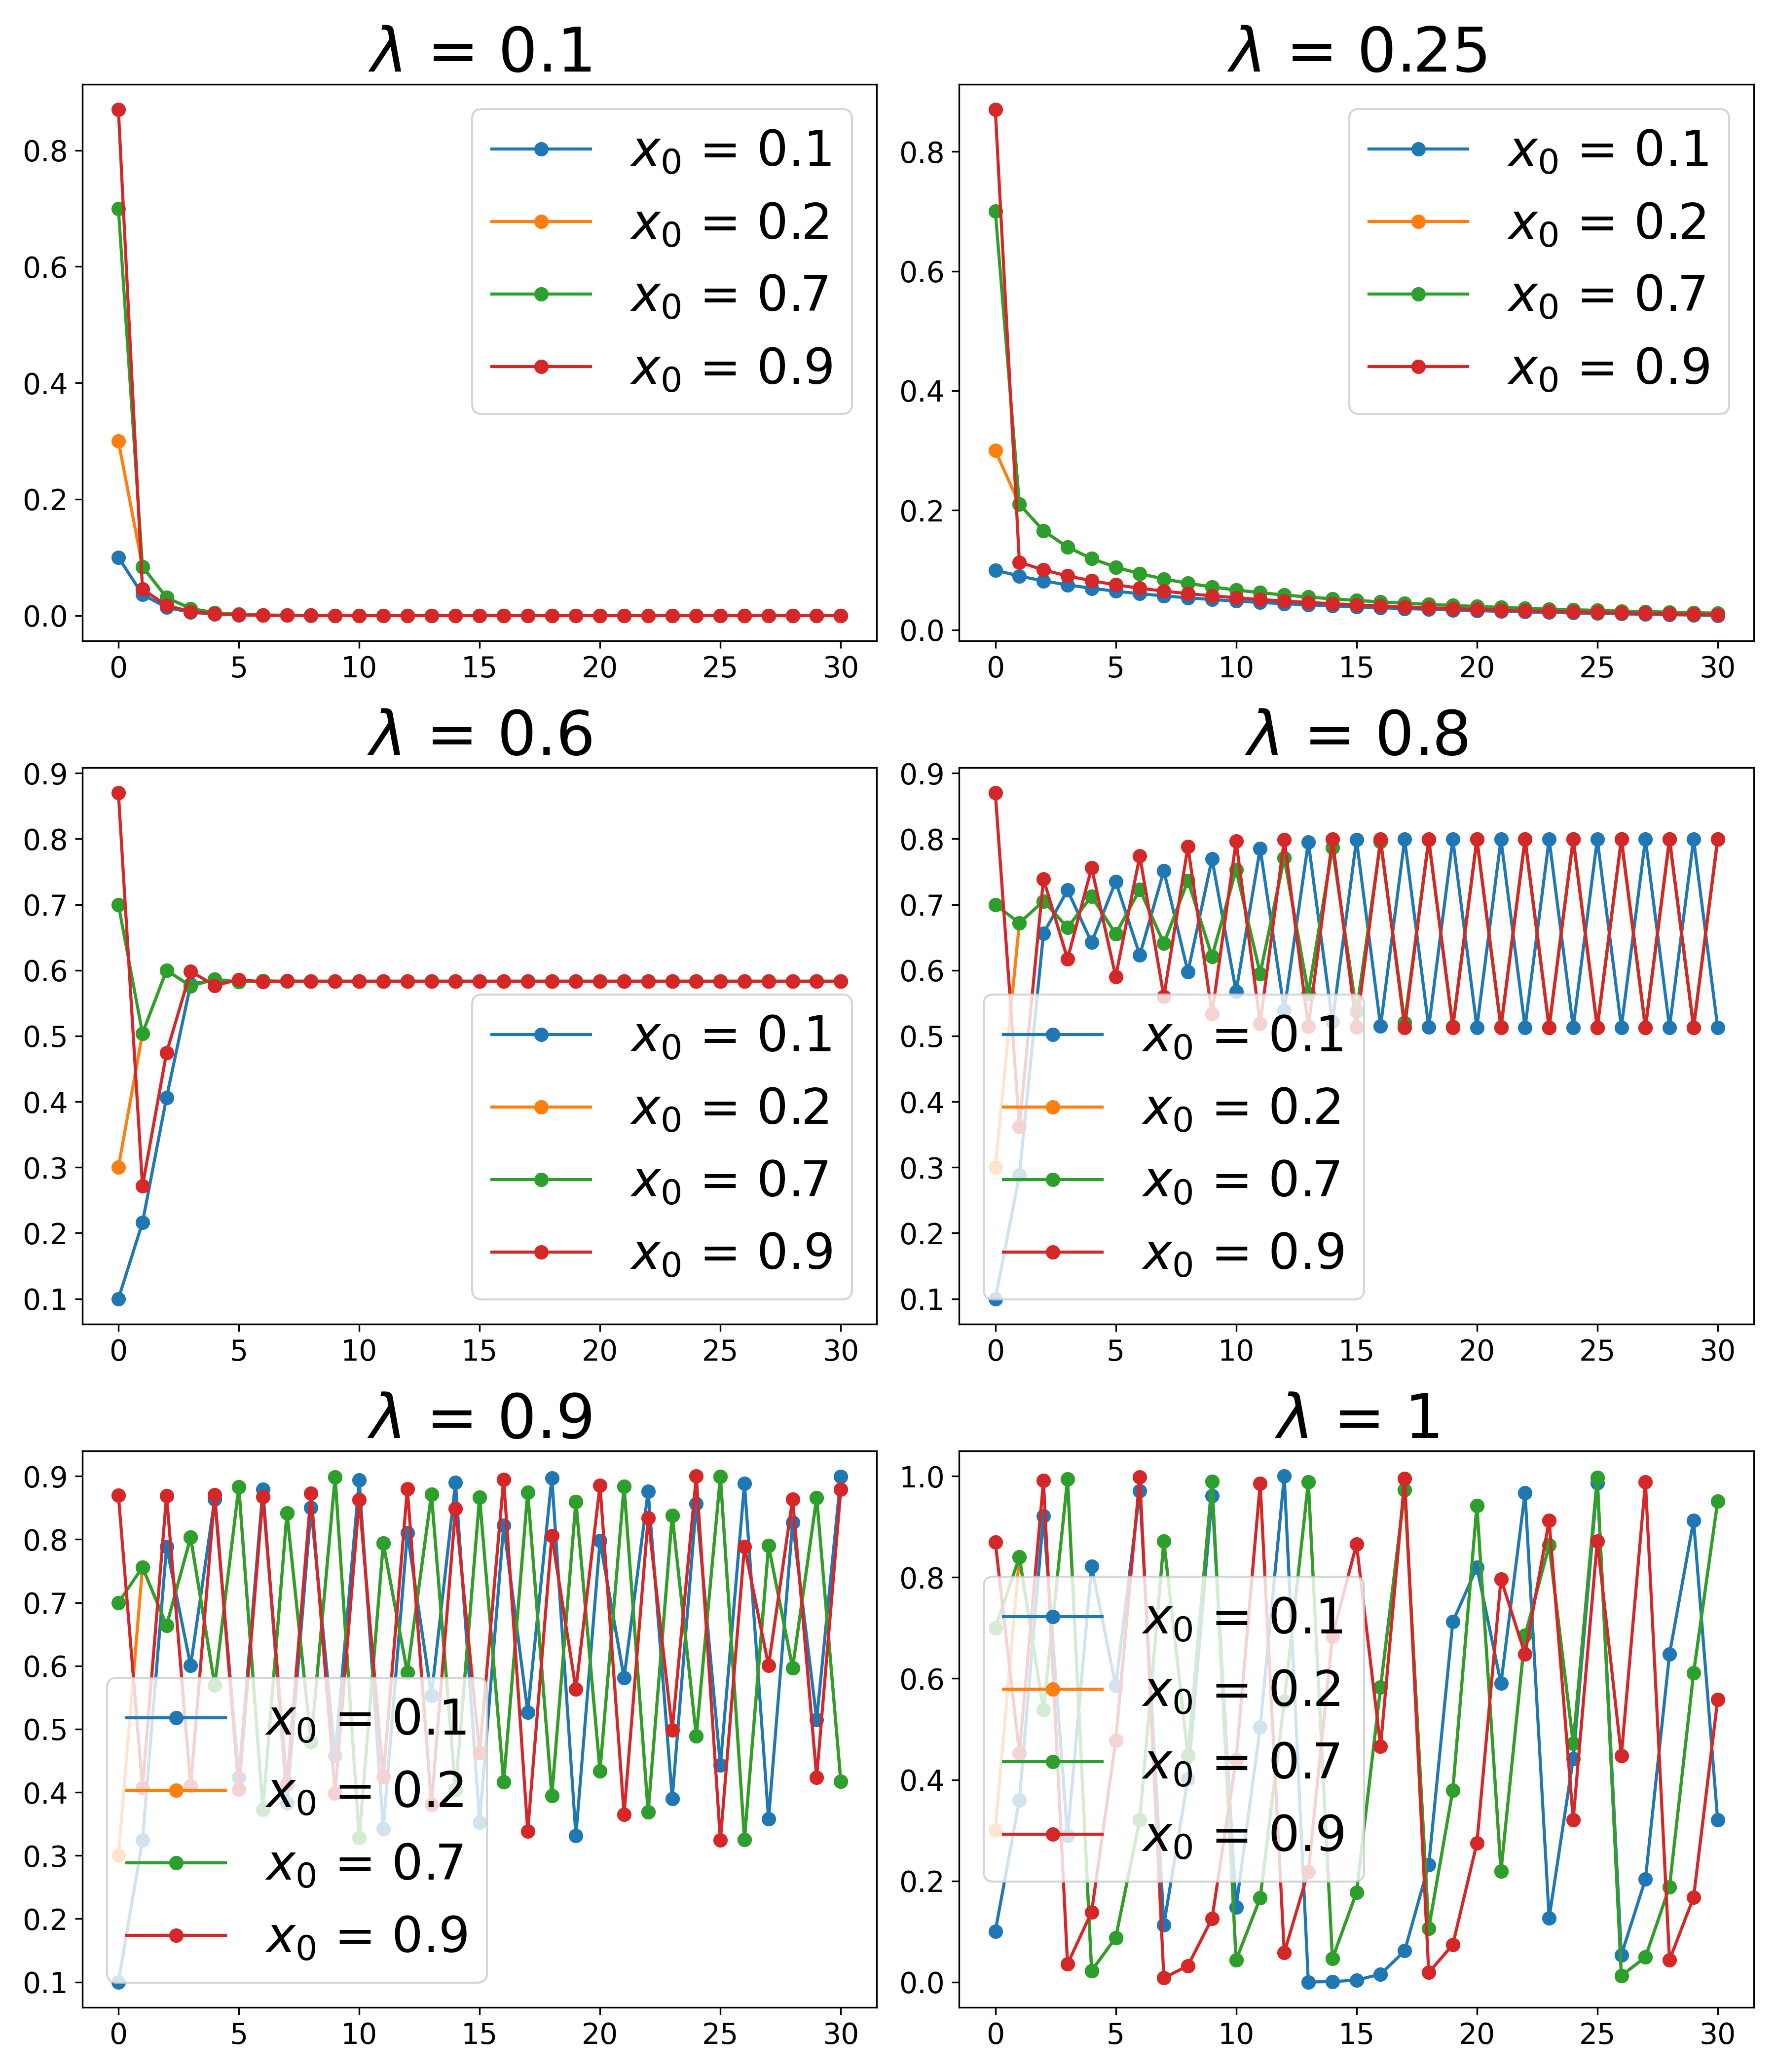
\includegraphics[width=\textwidth]{./figures/various_iterating_logistic_map.png}
	\caption{Iterating the logistic map with different initial values and $\lambda$. All graphs are produced by setting a $x_0$ and $\lambda$, and iterating $x_{n+1} = L_{\lambda}(x_n)$, and plotting all $x_n$ values respect to iteration number $n$.}
\end{figure}

There are several immediate observations upon looking at the figure \ref{fig:various_iter_logistic}.
When $\lambda = 0.1$ and $0.25$, it seems $\lim_{n \rightarrow \infty} x_n = 0$ regardless of the value of $x_0$.
For $\lambda = 0.6$, $\lim_{n \rightarrow \infty} x_n = l \neq 0$. 
(We can show that, after more tools a developped in the next sessions, $l = \frac{7}{12}$). 

When $\lambda = 0.8$, $x_n$ no longer converges, instead it seems to oscillate in a stable two orbit. When $\lambda = 0.9$ and $\lambda = 1$, it is not clear that if $x_n$ has any stable orbits or sensible patterns, and the best epithed for them would be `chaotic'.
A rigorous topological definition for chaos will be provided in the following session.

For all cases it seems like any initial condtion, $x_0$, upon iteration, will eventually tend to some common dynamical behavior depending only on $\lambda$.
The scatter plot, figure \ref{fig:logistic bifurcation overview}, is produced to capture the behavior of $x_n$ as $n \rightarrow \infty$ for $0 \leq \lambda \leq 1$. 
Two zoomed in figure around the area of bifurcation are also produced.

These pictures of bifurcation are indeed spectacular. 
There is one single stable orbit until $\lambda = 0.75$, after which a stable two cycles appears.
The two cycle bifurcated to 4 cycles, $2^3$ cycles, $2^n$ cycles, but after some threshold around $\lambda = 0.88$, there are no longer clear stable cycles and all that is left are chaos. 


\begin{figure}[htbp]
	\centering
	\label{fig:logistic bifurcation overview}
	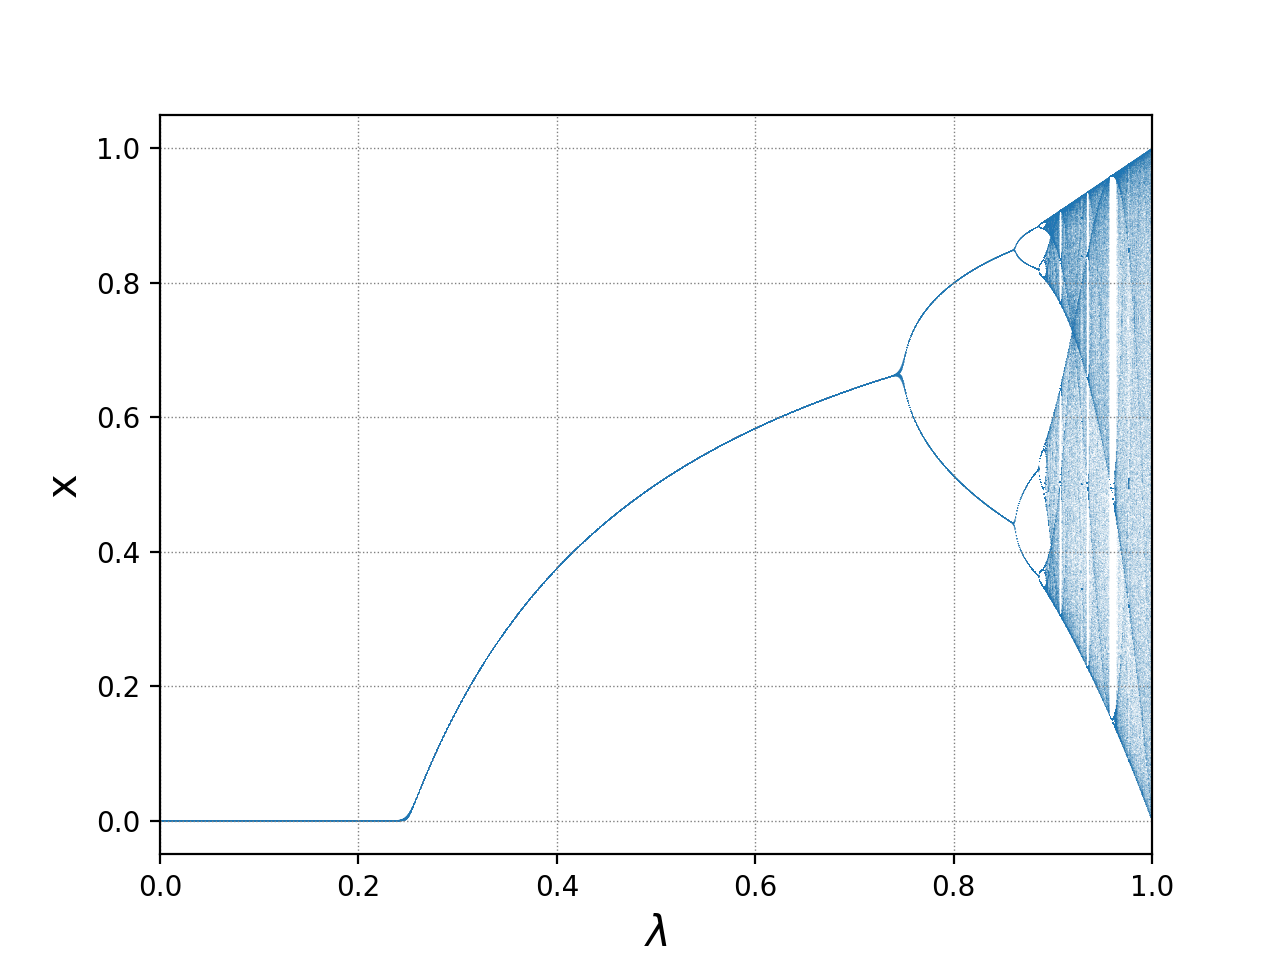
\includegraphics[width=\textwidth]{./figures/l_bifurcation_overview.png}
	\caption{For each $\lambda \in [0,1]$, $x_0$ is set to $0.5$, and the value of each iteration of $x_{n+1} = L_{\lambda}(x_n)$ was plotted at the coordinate $(\lambda, x_{n+1})$ as a faint blue dot. 
	The first 100 iteration was discarded, and 1500 iterations were plotted for each value of $\lambda$.}
\end{figure}

\begin{figure}[htbp]
	\centering
	\label{fig:logistic_bifurcation_zoom_1}
	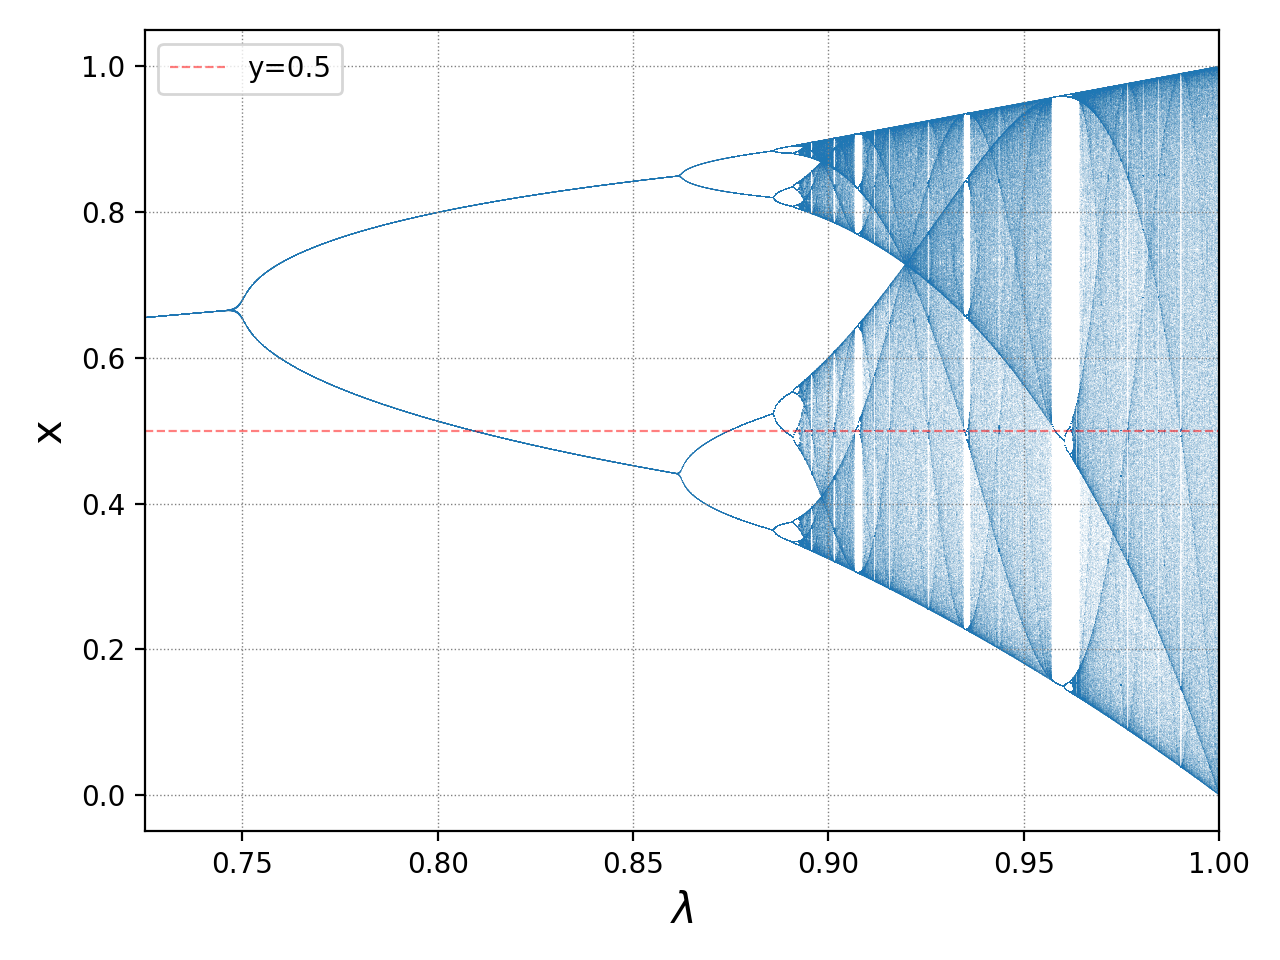
\includegraphics[width=\textwidth]{./figures/l_bifurcation_zoom_1.png}
	\caption{Zooming in the figure \ref{fig:logistic bifurcation overview} at the interval $0.5 \leq \lambda \leq 1$.}
\end{figure}

% TODO: caption non finished
\begin{figure}[htbp]
	\centering
	\label{fig:logistic_bifurcation_zoom_2}
	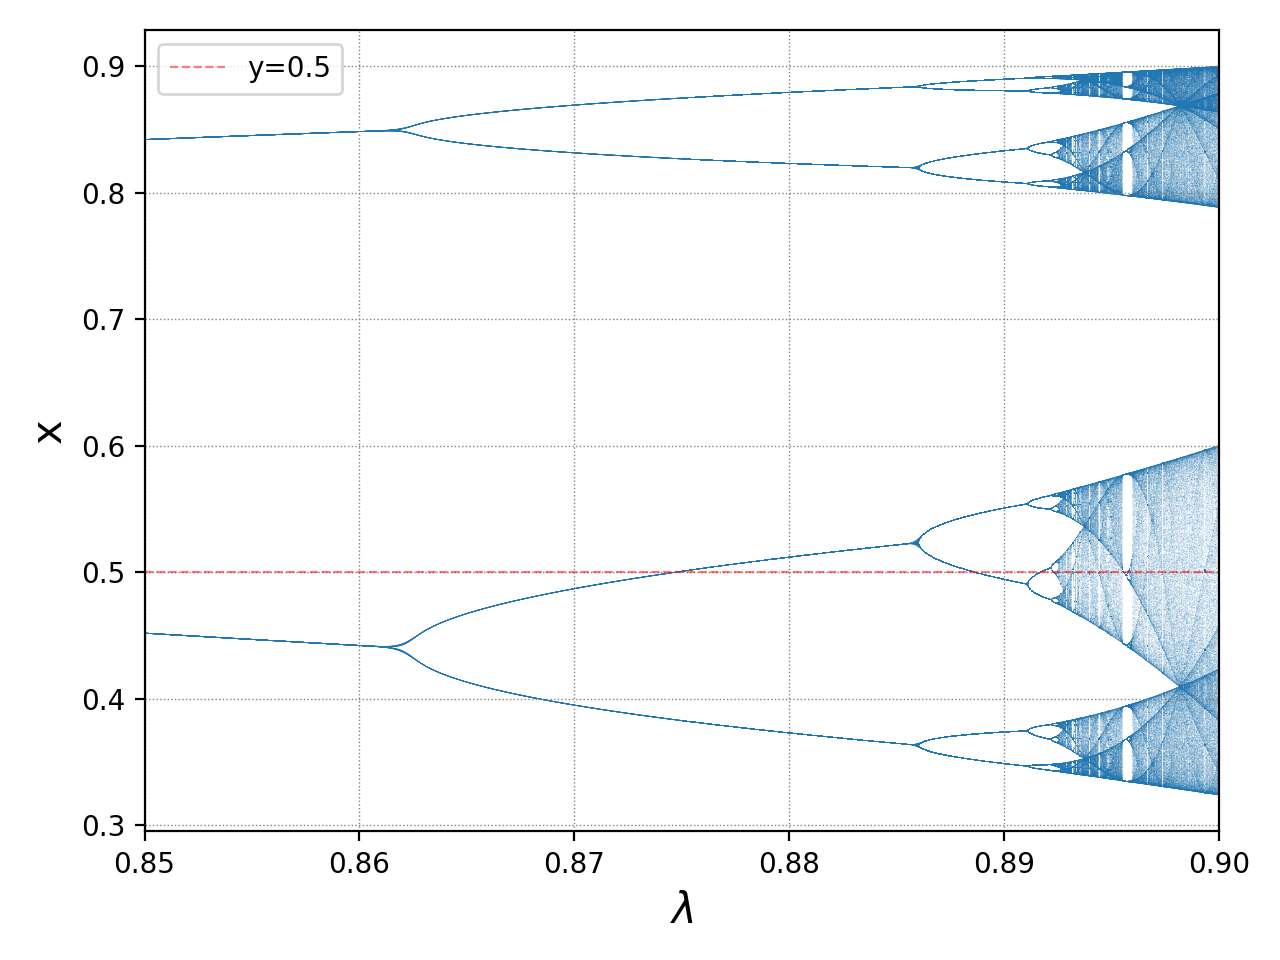
\includegraphics[width=\textwidth]{./figures/l_bifurcation_zoom_2.png}
	\caption{Zooming in the figure \ref{fig:logistic bifurcation overview} at the interval $0.5 \leq \lambda \leq 1$.}
\end{figure}

\begin{observation}[Logistic Bifurcation]\label{th:logistic_bifurcation}
	Let $f_{\lambda} = \lambda 4x(1-x) $ be the logistic function with a parameter $\lambda$, which takes value from $0$ to $1$. 
	Notice the $f_{;}$ attains the unique maximum 1 at $\mx = \frac{1}{2}$, and $f_{\lambda}(\mx) = \lambda$.
	Let $x_0 \in [0,1]$ and generate sequence of $x_i$ such that $x_{i+1} = f_{\lambda}(x_i)$.
	The behavior of $x_i$ varies as $\lambda$ increases from 0 to 1. Let $0 < B_0 < B_1 < \cdots < B_{\infty} < 1$ be the value of $\lambda$ at which the behavior of $x_i$ changes.

	\begin{enumerate}
		\item For all $0 < \lambda < B_0$, $x_i$ has a unique and stable one cycle at $x=0$.
		\item For all $B_0 <\lambda < B_1 = \frac{3}{4}$, the one cycle at $x=0$ is no longer stable, but a new stable one-cycle were developped.
		\item When $\lambda = \mx = \frac{1}{2}< B_1$, the one circle attains superstability. Define $A_1 = \mx$ .
		\item When $\lambda > B_2$, the one cycle is no longer stable. Precisely at the point when the one cycle fails to be stable, a stable two cycle appears.
		\item At some $B_2 <A_2 < B_3$ the 2 cycle enjoys superstability, and one of the value of the $2$ cycle must be $\mx$.
		\item Similar trends continue. When $\lambda > B_k$, the previous $2^{k-2}$ cycle becomes unstable and a new stable $2^{k-1}$ cycle were developped. One of the value of the cycle must be $\mx$ at some $\lambda, B_k <\lambda < B_{k+1}$, and at this point the cycle enjoys superstability.
		\item $B_{\infty} < 1$, and for most of the value after $B_{\infty}$ $x_i$ behaves. 
		\item Specifically, at $\lambda = 1$, $x_i$ has chaotic behavior defined in TODO
	\end{enumerate}

\end{observation}

\section{Single Nodal Functions Give Rise to Bifurcations}

It is very common for a mathematic model to consist, at least in parts, of iterations of some functions.
For the sake of simplicity and generosity, assume the value of our interest is $x_i$ is modelled by the simple recursive relations $f$ with the parameter $\lambda$. With appropriate rescaling, we assume moreover $x_i \in [0,1], \lambda \in [0,1]$ and $f: [0,1] \rightarrow [0,1]$:

\begin{equation}
	x_{i+1}=\lambda f(x_i)
\end{equation}
The presice definition of $f$ and $\lambda$, of course, depend on the behavior of the object in interest and is not of our relevence here.

%TODO: Is single nodal the correct term?
% TODO: add figure single nodal function
It may seem like nothing can be said by such a generalised model. However, with one more modest restriction that $f$ is single nodal, which just means the profile of $f$ is similar to figure TODO:, $x_i$ will exhibit the surprising structure of bifurcation, showing in figure (TODO: add figure)

% TODO: what is the correct term of B_1 A_1 etc?
\begin{thm}[Bifurcation]\label{th:general_bifurcation}
	Let $f_{\lambda}: [0,1] \rightarrow [0,1] $ be a single nodal function with a parameter $\lambda$, which takes value from $0$ to $1$. 
	Assume the $f_{1}$ attains the unique maximum 1 at $\mx$.
	Let $x_0 \in [0,1]$ and generate sequence of $x_i$ such that $x_{i+1} = f_{\lambda}(x_i)$.
	The behavior of $x_i$ varies as $\lambda$ increases from 0 to 1. Let $0 < B_0 < B_1 < \cdots < B_{\infty} < 1$ be the value of $\lambda$ at which the behavior of $x_i$ changes.

	\begin{enumerate}
		\item For all $0 <\lambda < B_1$, $x_i$ has a unique and stable one-cycle
		\item When $\lambda = \mx < B_1$, the one circle attains superstability precisely at $\mx$. Define $A_1 = \mx$ .
		\item When $\lambda > B_2$, the one cycle is no longer stable. Precisely at the point when the one cycle fails to be stable, a stable two cycle appears.
		\item At some $B_2 <A_2 < B_3$ the 2 cycle enjoys superstability, and one of the value of the $2$ cycle must be $\mx$.
		\item Similar trends continue. When $\lambda > B_k$, the previous $2^{k-2}$ cycle becomes unstable and a new stable $2^{k-1}$ cycle were developped. One of the value of the cycle must be $\mx$ at some $\lambda, B_k <\lambda < B_{k+1}$, and at this point the cycle enjoys superstability.
		\item $B_{\infty} < 1$, and for most of the value after $B_{\infty}$ $x_i$ behaves. 
		\item Specifically, at $\lambda = 1$, $x_i$ has chaotic behavior defined in TODO
	\end{enumerate}

\end{thm}

Here is the precise definition for a function to be single nodal:

% TODO: is a circle signle nodal? for all $\lambda$ the cicle has exactly on stable one-cycle. 
% TODO: are there more examples like the circle? Or are there more examples of similar function that only exhibit finite Bifurcations?

\begin{defn}
	A function $f: [0,1] \rightarrow [0,1]$ is single nodal if 
	\begin{enumerate}
		\item $f$ is piecewise $C^2$, that is, doubly differentiable with continuous second derivative
		\item $f$ has a unique and differentiable maximum attained at $f(\mx) = 1$ and $f'$ is continuous at $\mx$.
% TODO: Do we need the condition that f has no other local maximum?
		\item $f(x) > 0$ and $f(1) = f(0) =0$
		\item $f(x)$ concave downwards, that is $f'' < 0$.
	\end{enumerate}

	This definition is modified from appendix A of Feigenbuam's paper \cite{F1}.
\end{defn}

Although theorem \ref{th:general_bifurcation} may seem extremely bold in claim, 

\printbibliography
\end{document}
